\section*{Post-Processing}


\begin{figure}[ht]
    \centering
    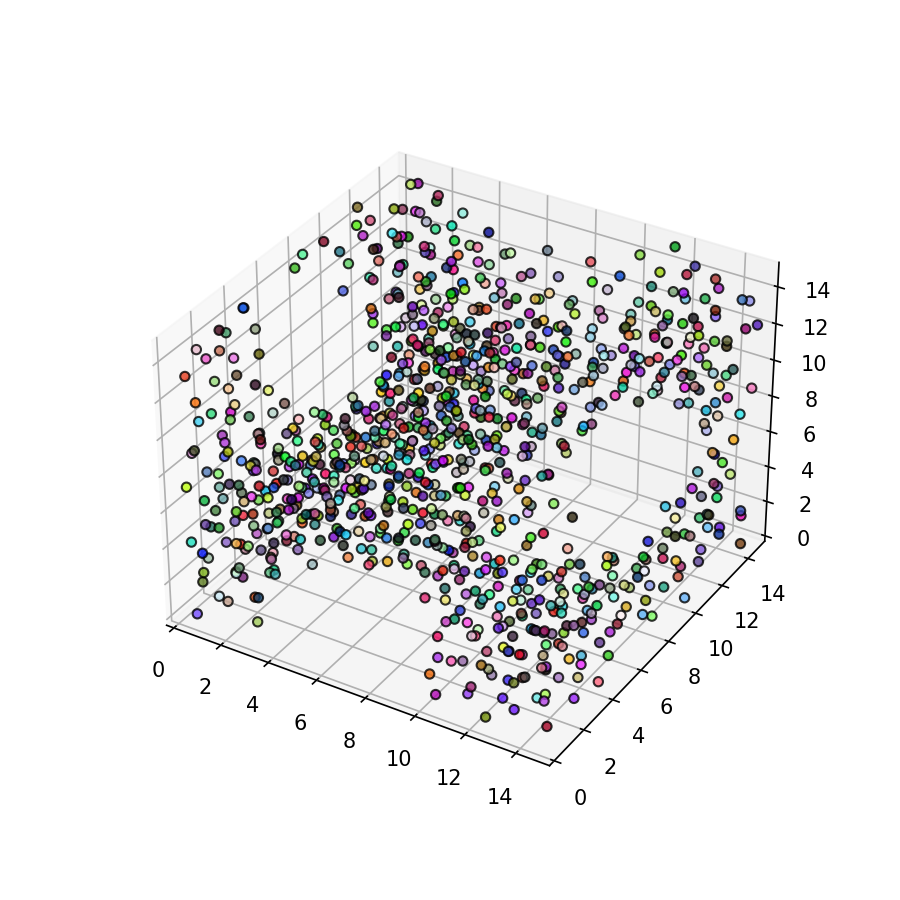
\includegraphics[width=1\textwidth]{figures/3d_plot_IC.png}
	\caption{Initial Condition for Molecular Dynamics Simulation with 1000 Particles at 300K}
	\label{3d_plot_IC}
\end{figure}

Figure \ref{3d_plot_IC} shows the initial condition which is generated from \texttt{ task2.py}. The positions are at a local minimum which is numerically obtained
by the \texttt{scipy.optimize.minimize()} funtcion with the conjugate gradient method. The CG method needs the gradient to obtain the minimum which is passed
as an argument to the function. Not visible in the figure above, are the initial velocites which are also randomly assigned to every particle with the \texttt{numpy.random.multivariate.normal()}
function. This initial condition, namely positions and velocities of each particle, are written to a txt file which is interpreted by pythonfile \texttt{task3.py}.
In said file the trajectories of all thsee particles are calculated by integration of Newtons equations of motion, this part is called the velocity verlet algorithm

\pagebreak

\begin{figure}[ht]
    \centering
    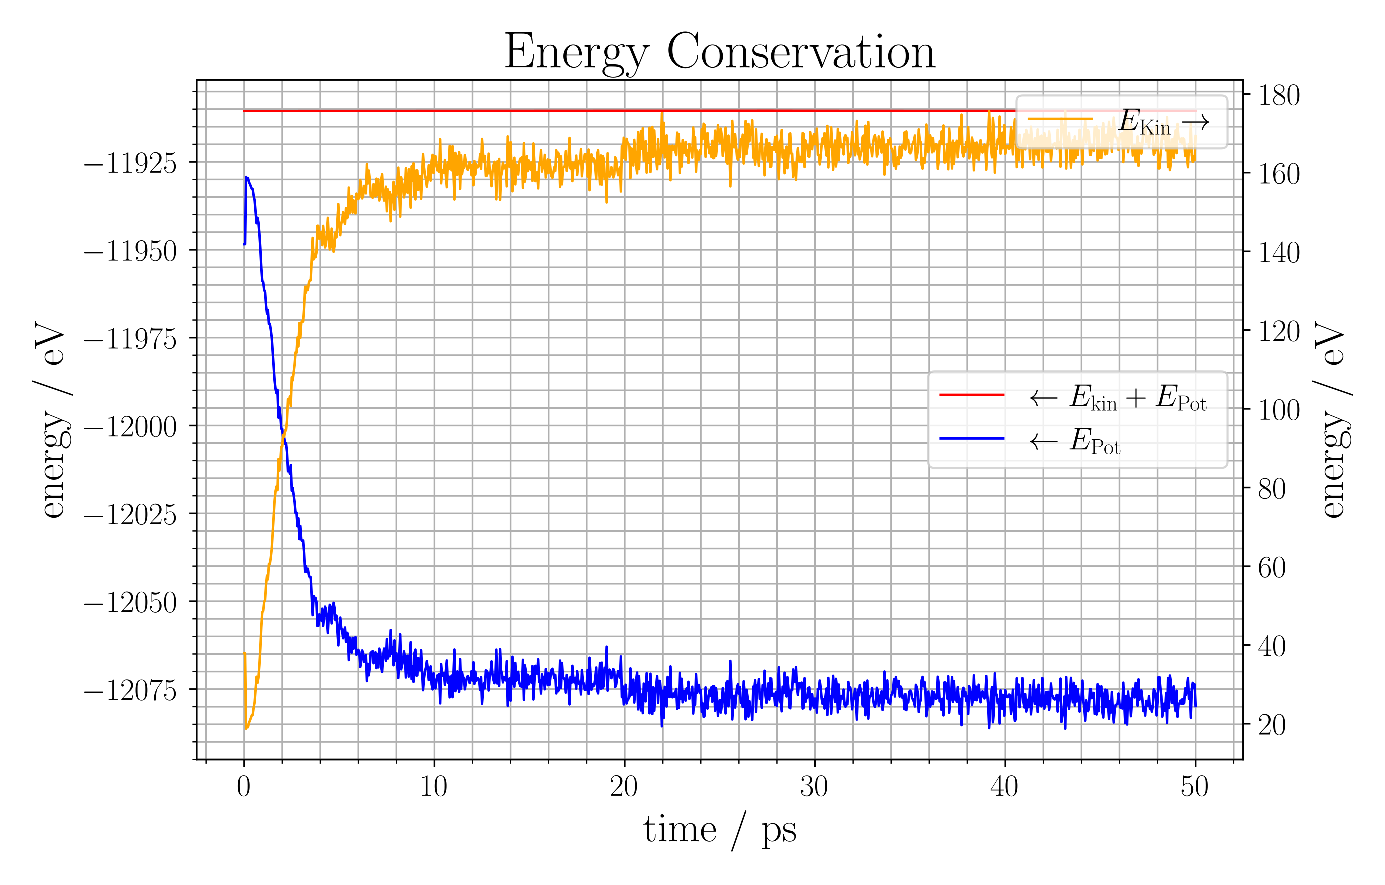
\includegraphics[width=1\textwidth]{figures/energy_conservation.eps}
	\caption{Energy Conservation Plot for $10^6$ timesteps of 0.5 femtoseconds}
	\label{energy_conservation_plot}
\end{figure}

In figure \ref{energy_conservation_plot} above, the energy conservation is shown. Since this molecular dynamics simulation result is obtained numerically,
errors are expected. The main error source being the velocity verlet algorithm, for the chosen timestep, the error is negligible. 
The timestep in this simulation was reduced until a reasonable energy conservation was observed. The timestep chosen was 0.05 femtoseconds. 

\pagebreak

\begin{figure}[ht]
    \centering
    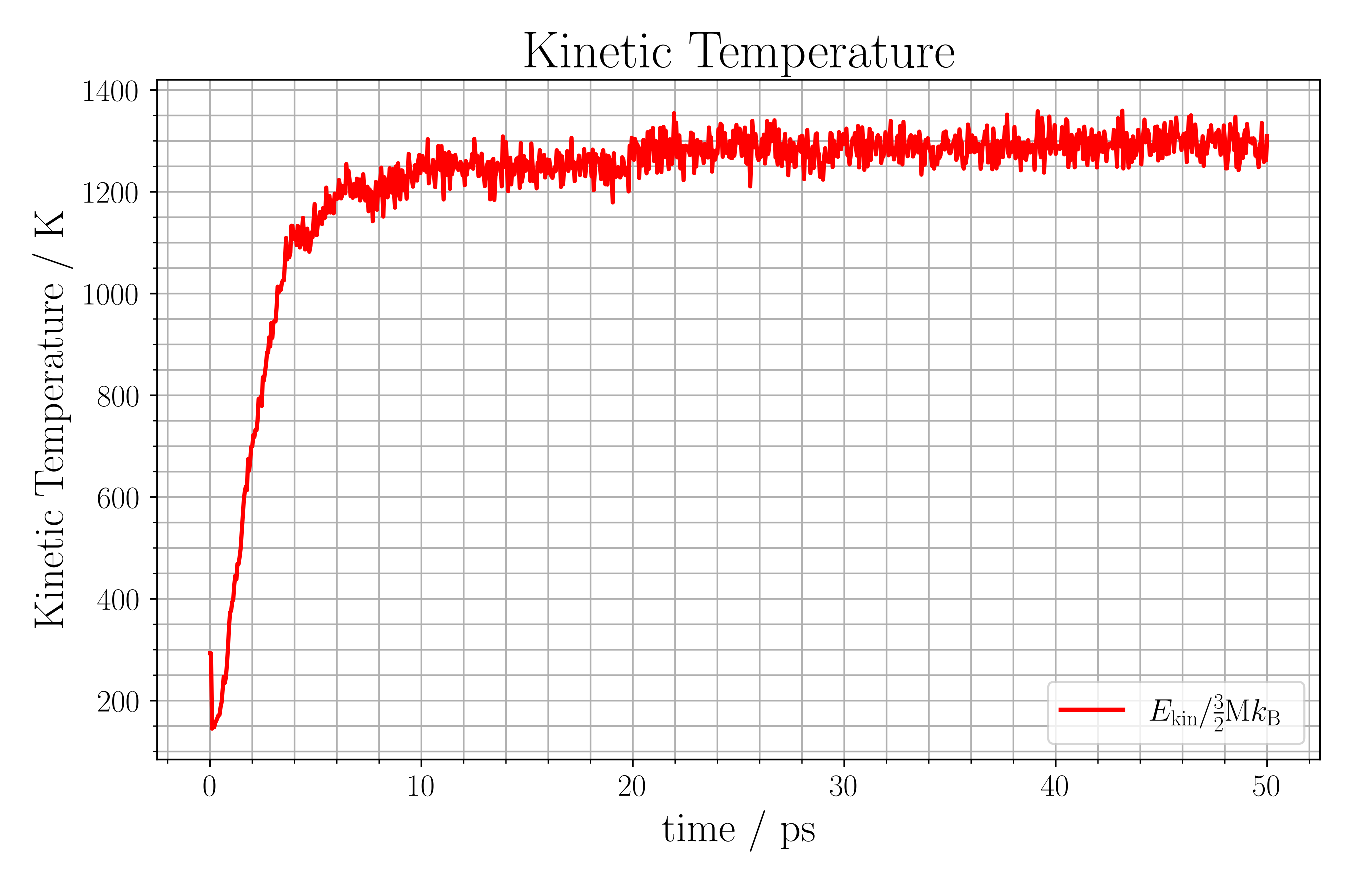
\includegraphics[width=1\textwidth]{figures/kin_temp.eps}
	\caption{Evolution of Kinetic Temperature for $10^6$ timesteps of 0.05 femtoseconds}
	\label{kin_temp_plot}
\end{figure}

In figure \ref{kin_temp_plot} the evolution of the kinetic temperature over the simulated time is plotted. At $t=0$, The kinetic temperature is at 300K, which
is in agreement with the velocities assigned in the initial conditions. The final state where potential and kinetic energy are not changing each other anymore, it reaches a
kinetic temperature of approximately 1300 Kelvin. \\

In order to obtain a specific heat, an approximation formula was provided, where 25 \% of the trajectory data, timewise, had to be neglected.
Said approximation formula yielded a quantity in $\mathrm{J} \slash \mathrm{K}$. If this quantity is divided by the mass of the system,
the weight specifc heat capacity can be obtained. This coefficient is used to model heat transport in solids as well as in fluids,
an example would be the poisson equation.The calculated specific heat capacity was 17.23887287974392 $\mathrm{J} \slash (\mathrm{kg} \cdot \mathrm{K})$. 
A comparable material would be hydrogen with a specific heat capacity of 10.16 $\mathrm{J} \slash (\mathrm{kg} \cdot \mathrm{K})$. However, other than
the equations of motion on the shape of the morse potential function, these simulation results do not have physical meaning.